\subsection{Yoctopuce Tips}

\subsubsection{Upgrade Yocto-Pictor firmwares}
\label{annex:yoctoUpdate} 

Please refer to the
\href{https://www.yoctopuce.com/EN/products/virtualhub/doc/VIRTHUB0.usermanual.html#CHAP3SEC4}
{yoctopuce documentation} in order to upgrade the firmwares.

% TODO:
% Note : the yoctopuce has to be powered by external source using input socket not usb
% screen yoctoUpdate.zip 

\subsubsection{How to catch debug informations}

The Yocto-Pictor is still a tool under development and some bugs may
sometimes show up. So when something wrong happens. For example the software is 
reporting an error relative to yocto or the behaviour is not the one expected. 
It could be helpful to join a \emph{memory dump} of the card to the issue
report. In order to get this file, here is the most common scenario:

\begin{enumerate}
	\item Something goes wrong with the card.

	\item Don't touch anything but hold on the Ybutton during 5 seconds 
		(see figure \ref{fig:ybutton}).

	\item Now, restart the system in order to get back the Wi-Fi connection 
		working.

	\item Go to the yoctopuce webpage (by typing : 10.42.0.X:4444 in the
		address bar of a web browser).

	\item Click successively on \emph{Configure} (on the row of
		\emph{Yocto-Pictor-Wifi}), then \emph{manage files} 
		(see \ref{fig:fileman}).

	\item You should see a row with \emph{dump.bin} under the column
		\emph{Path/name}.
		Download this file, using \emph{right click} and \emph{Download
		Linked File}.
		(see \ref{fig:downloadDump}).

	\item Finally click on \emph{remove} to delete the file in order to avoid
		eventual future confusion.
\end{enumerate}

For convenience, you can name the file with your initials, the date and
an error reference if there is one. Also, please mind to always send this 
file with an explanation of the issue or the error logs.

\begin{figure}[H]
  \centering
  \begin{minipage}[b]{0.40\textwidth}
	  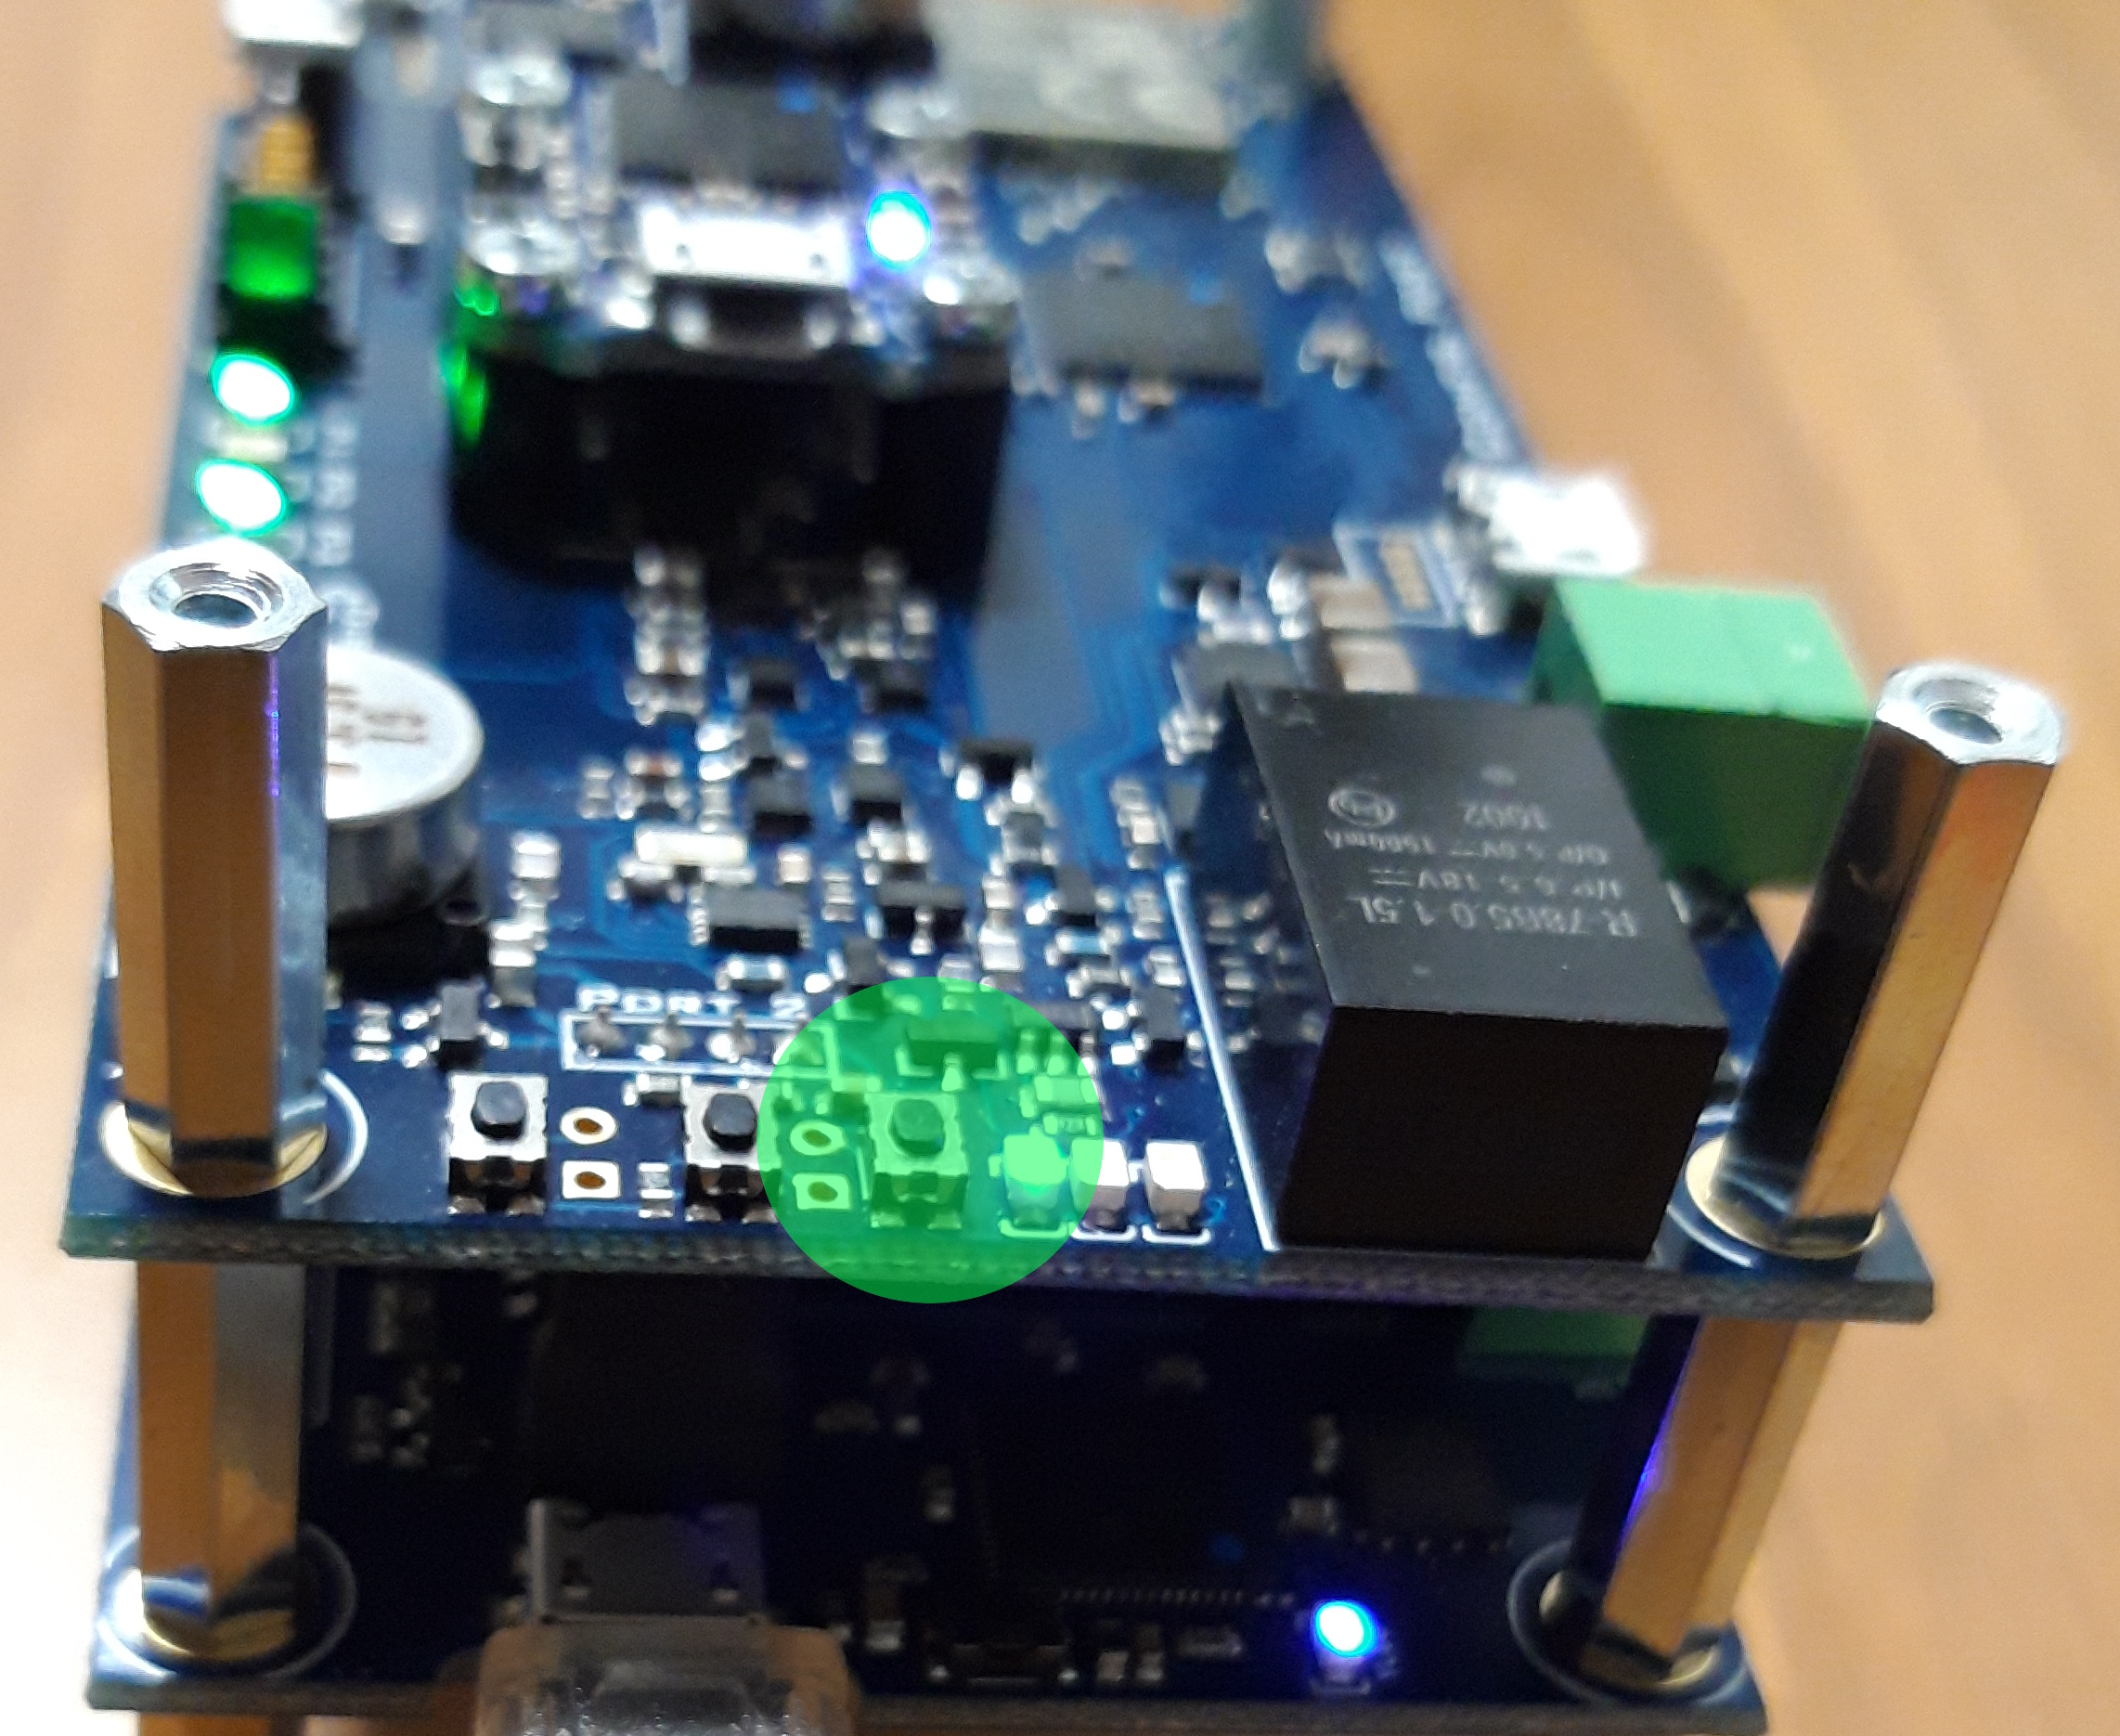
\includegraphics[scale=.09]{images/yoctopuce_bug1.jpg}
	  \caption{Highlighted \emph{YButton}}
	  \label{fig:ybutton}
  \end{minipage}
  \hfill
	\vspace{15pt}
  \begin{minipage}[b]{0.50\textwidth}
	  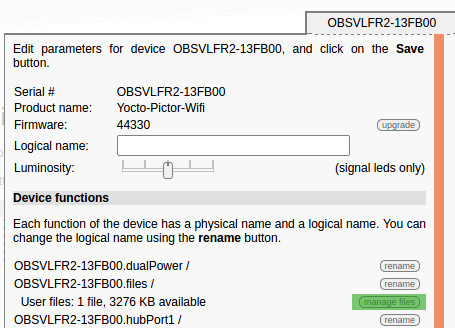
\includegraphics[scale=.54]{images/yoctopuce_bug2.jpg}
	  \caption{Hightlighted \emph{file manager}}
	  \label{fig:fileman}
  \end{minipage}
  \begin{minipage}[b]{0.50\textwidth}
	  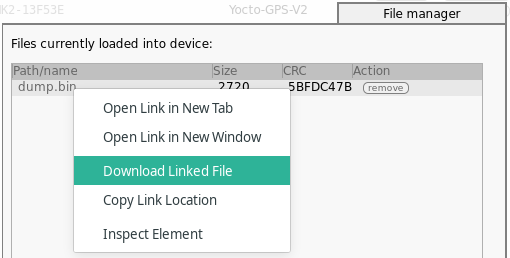
\includegraphics[scale=.54]{images/yoctopuce_bug3.png}
	  \caption{Download \emph{dump.bin}}
	  \label{fig:downloadDump}
  \end{minipage}
\end{figure}
